% Created by tikzDevice version 0.12.6 on 2026-02-22 21:44:02
% !TEX encoding = UTF-8 Unicode
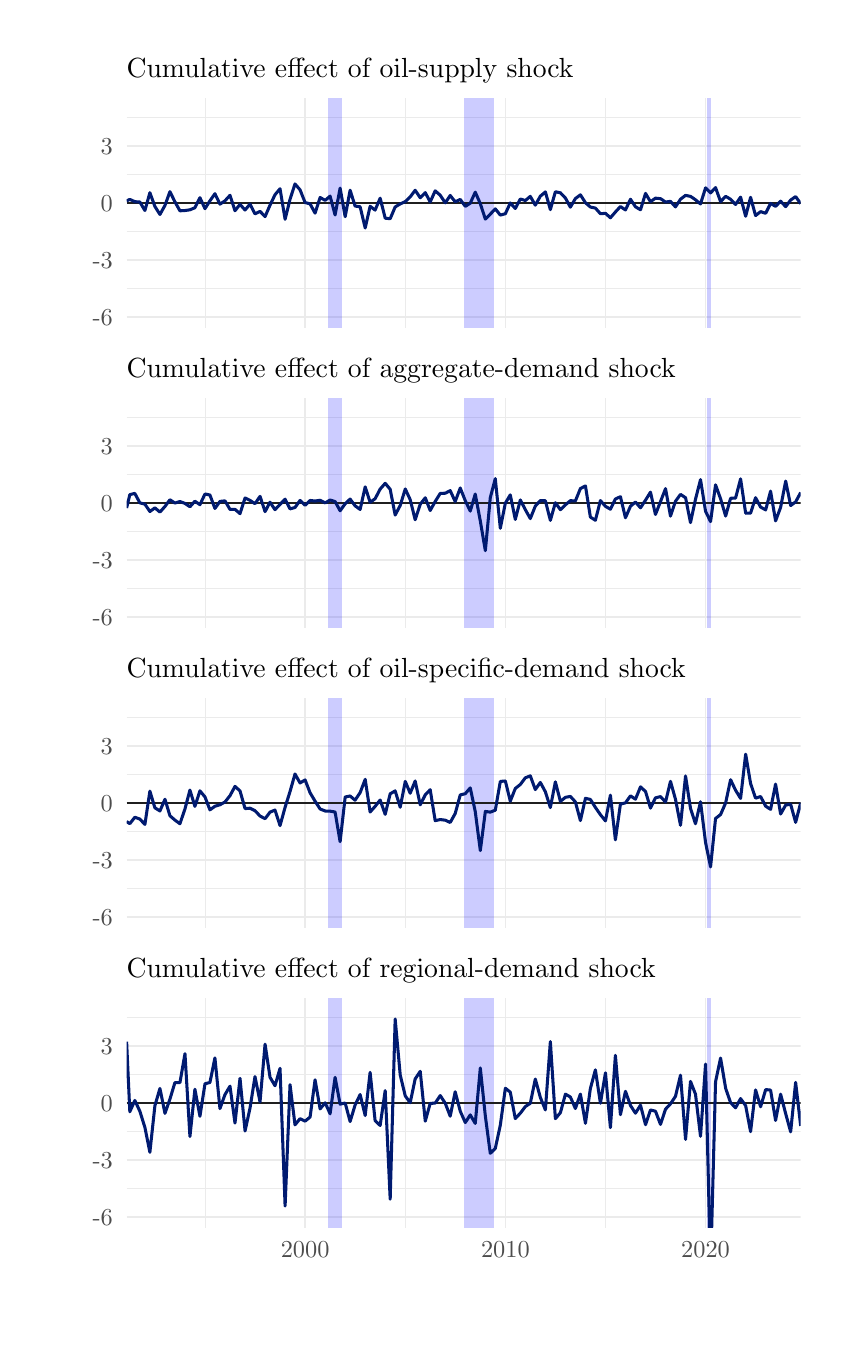
\begin{tikzpicture}[x=1pt,y=1pt]
\definecolor{fillColor}{RGB}{255,255,255}
\path[use as bounding box,fill=fillColor,fill opacity=0.00] (0,0) rectangle (290.32,469.75);
\begin{scope}
\path[clip] ( 35.75,361.36) rectangle (279.32,444.42);
\definecolor{drawColor}{gray}{0.92}

\path[draw=drawColor,line width= 0.3pt,line join=round] ( 35.75,375.44) --
	(279.32,375.44);

\path[draw=drawColor,line width= 0.3pt,line join=round] ( 35.75,396.03) --
	(279.32,396.03);

\path[draw=drawColor,line width= 0.3pt,line join=round] ( 35.75,416.62) --
	(279.32,416.62);

\path[draw=drawColor,line width= 0.3pt,line join=round] ( 35.75,437.22) --
	(279.32,437.22);

\path[draw=drawColor,line width= 0.3pt,line join=round] ( 64.07,361.36) --
	( 64.07,444.42);

\path[draw=drawColor,line width= 0.3pt,line join=round] (136.43,361.36) --
	(136.43,444.42);

\path[draw=drawColor,line width= 0.3pt,line join=round] (208.78,361.36) --
	(208.78,444.42);

\path[draw=drawColor,line width= 0.6pt,line join=round] ( 35.75,365.14) --
	(279.32,365.14);

\path[draw=drawColor,line width= 0.6pt,line join=round] ( 35.75,385.73) --
	(279.32,385.73);

\path[draw=drawColor,line width= 0.6pt,line join=round] ( 35.75,406.33) --
	(279.32,406.33);

\path[draw=drawColor,line width= 0.6pt,line join=round] ( 35.75,426.92) --
	(279.32,426.92);

\path[draw=drawColor,line width= 0.6pt,line join=round] (100.25,361.36) --
	(100.25,444.42);

\path[draw=drawColor,line width= 0.6pt,line join=round] (172.61,361.36) --
	(172.61,444.42);

\path[draw=drawColor,line width= 0.6pt,line join=round] (244.95,361.36) --
	(244.95,444.42);
\definecolor{fillColor}{RGB}{0,0,255}

\path[fill=fillColor,fill opacity=0.20] (108.66,361.36) rectangle (113.52,444.42);

\path[fill=fillColor,fill opacity=0.20] (157.52,361.36) rectangle (168.37,444.42);

\path[fill=fillColor,fill opacity=0.20] (245.57,361.36) rectangle (246.76,444.42);
\definecolor{drawColor}{gray}{0.12}

\path[draw=drawColor,line width= 0.6pt,line join=round] ( 35.75,406.33) -- (279.32,406.33);
\definecolor{drawColor}{RGB}{0,26,112}

\path[draw=drawColor,line width= 1.1pt,line join=round] ( 35.75,407.13) --
	( 36.91,407.69) --
	( 38.72,406.87) --
	( 40.54,406.75) --
	( 42.36,403.67) --
	( 44.16,410.11) --
	( 45.97,405.14) --
	( 47.79,402.25) --
	( 49.61,405.51) --
	( 51.40,410.49) --
	( 53.20,406.84) --
	( 55.02,403.57) --
	( 56.84,403.67) --
	( 58.63,403.93) --
	( 60.43,404.67) --
	( 62.25,408.31) --
	( 64.07,404.34) --
	( 65.86,407.18) --
	( 67.66,409.75) --
	( 69.48,405.97) --
	( 71.30,407.20) --
	( 73.11,409.17) --
	( 74.91,403.60) --
	( 76.73,405.89) --
	( 78.55,403.85) --
	( 80.34,405.99) --
	( 82.14,402.45) --
	( 83.96,403.38) --
	( 85.78,401.47) --
	( 87.57,405.62) --
	( 89.37,409.37) --
	( 91.19,411.54) --
	( 93.02,400.50) --
	( 94.80,407.73) --
	( 96.60,413.28) --
	( 98.42,411.15) --
	(100.25,406.56) --
	(102.05,406.07) --
	(103.85,402.72) --
	(105.67,408.38) --
	(107.50,407.34) --
	(109.28,408.88) --
	(111.08,402.06) --
	(112.90,411.77) --
	(114.73,401.43) --
	(116.51,411.02) --
	(118.31,405.28) --
	(120.13,405.03) --
	(121.96,397.36) --
	(123.74,405.21) --
	(125.54,403.83) --
	(127.37,408.13) --
	(129.19,400.90) --
	(130.99,400.71) --
	(132.79,404.96) --
	(134.62,406.06) --
	(136.44,406.89) --
	(138.22,408.60) --
	(140.02,410.99) --
	(141.85,408.29) --
	(143.67,410.14) --
	(145.45,406.76) --
	(147.25,410.79) --
	(149.08,409.19) --
	(150.90,406.45) --
	(152.68,409.11) --
	(154.48,406.82) --
	(156.31,407.68) --
	(158.13,405.18) --
	(159.93,406.32) --
	(161.73,410.32) --
	(163.56,406.15) --
	(165.38,400.58) --
	(167.16,402.36) --
	(168.97,404.28) --
	(170.79,402.02) --
	(172.61,402.51) --
	(174.39,406.41) --
	(176.20,404.41) --
	(178.02,407.84) --
	(179.84,407.28) --
	(181.62,408.79) --
	(183.43,405.61) --
	(185.25,408.85) --
	(187.07,410.39) --
	(188.87,404.00) --
	(190.68,410.45) --
	(192.50,410.08) --
	(194.32,408.17) --
	(196.10,404.87) --
	(197.91,407.99) --
	(199.73,409.34) --
	(201.55,406.49) --
	(203.33,404.94) --
	(205.14,404.55) --
	(206.96,402.52) --
	(208.78,402.65) --
	(210.57,401.05) --
	(212.37,403.13) --
	(214.19,405.12) --
	(216.01,403.88) --
	(217.82,407.76) --
	(219.62,405.03) --
	(221.44,403.94) --
	(223.26,409.85) --
	(225.05,406.86) --
	(226.85,408.14) --
	(228.67,407.96) --
	(230.49,406.74) --
	(232.28,406.98) --
	(234.08,404.98) --
	(235.90,407.76) --
	(237.72,409.15) --
	(239.51,408.79) --
	(241.31,407.56) --
	(243.13,406.04) --
	(244.95,411.87) --
	(246.76,410.04) --
	(248.56,411.95) --
	(250.38,406.89) --
	(252.21,408.80) --
	(253.99,407.75) --
	(255.79,405.86) --
	(257.61,408.51) --
	(259.44,401.59) --
	(261.22,408.45) --
	(263.02,401.85) --
	(264.84,403.27) --
	(266.67,402.67) --
	(268.45,406.23) --
	(270.25,405.18) --
	(272.07,407.05) --
	(273.90,405.06) --
	(275.70,407.47) --
	(277.50,408.70) --
	(279.32,406.16);
\end{scope}
\begin{scope}
\path[clip] (  0.00,  0.00) rectangle (290.32,469.75);
\definecolor{drawColor}{gray}{0.30}

\node[text=drawColor,anchor=base east,inner sep=0pt, outer sep=0pt, scale=  0.88] at ( 30.80,362.11) {-6};

\node[text=drawColor,anchor=base east,inner sep=0pt, outer sep=0pt, scale=  0.88] at ( 30.80,382.70) {-3};

\node[text=drawColor,anchor=base east,inner sep=0pt, outer sep=0pt, scale=  0.88] at ( 30.80,403.30) {0};

\node[text=drawColor,anchor=base east,inner sep=0pt, outer sep=0pt, scale=  0.88] at ( 30.80,423.89) {3};
\end{scope}
\begin{scope}
\path[clip] (  0.00,  0.00) rectangle (290.32,469.75);
\definecolor{drawColor}{RGB}{0,0,0}

\node[text=drawColor,anchor=base west,inner sep=0pt, outer sep=0pt, scale=  1.00] at ( 35.75,451.87) {Cumulative effect of oil-supply shock};
\end{scope}
\begin{scope}
\path[clip] ( 35.75,252.97) rectangle (279.32,336.03);
\definecolor{drawColor}{gray}{0.92}

\path[draw=drawColor,line width= 0.3pt,line join=round] ( 35.75,267.04) --
	(279.32,267.04);

\path[draw=drawColor,line width= 0.3pt,line join=round] ( 35.75,287.64) --
	(279.32,287.64);

\path[draw=drawColor,line width= 0.3pt,line join=round] ( 35.75,308.23) --
	(279.32,308.23);

\path[draw=drawColor,line width= 0.3pt,line join=round] ( 35.75,328.82) --
	(279.32,328.82);

\path[draw=drawColor,line width= 0.3pt,line join=round] ( 64.07,252.97) --
	( 64.07,336.03);

\path[draw=drawColor,line width= 0.3pt,line join=round] (136.43,252.97) --
	(136.43,336.03);

\path[draw=drawColor,line width= 0.3pt,line join=round] (208.78,252.97) --
	(208.78,336.03);

\path[draw=drawColor,line width= 0.6pt,line join=round] ( 35.75,256.75) --
	(279.32,256.75);

\path[draw=drawColor,line width= 0.6pt,line join=round] ( 35.75,277.34) --
	(279.32,277.34);

\path[draw=drawColor,line width= 0.6pt,line join=round] ( 35.75,297.93) --
	(279.32,297.93);

\path[draw=drawColor,line width= 0.6pt,line join=round] ( 35.75,318.53) --
	(279.32,318.53);

\path[draw=drawColor,line width= 0.6pt,line join=round] (100.25,252.97) --
	(100.25,336.03);

\path[draw=drawColor,line width= 0.6pt,line join=round] (172.61,252.97) --
	(172.61,336.03);

\path[draw=drawColor,line width= 0.6pt,line join=round] (244.95,252.97) --
	(244.95,336.03);
\definecolor{fillColor}{RGB}{0,0,255}

\path[fill=fillColor,fill opacity=0.20] (108.66,252.97) rectangle (113.52,336.03);

\path[fill=fillColor,fill opacity=0.20] (157.52,252.97) rectangle (168.37,336.03);

\path[fill=fillColor,fill opacity=0.20] (245.57,252.97) rectangle (246.76,336.03);
\definecolor{drawColor}{gray}{0.12}

\path[draw=drawColor,line width= 0.6pt,line join=round] ( 35.75,297.93) -- (279.32,297.93);
\definecolor{drawColor}{RGB}{0,26,112}

\path[draw=drawColor,line width= 1.1pt,line join=round] ( 35.75,296.18) --
	( 36.91,301.00) --
	( 38.72,301.46) --
	( 40.54,298.03) --
	( 42.36,297.57) --
	( 44.16,294.91) --
	( 45.97,296.23) --
	( 47.79,294.70) --
	( 49.61,296.74) --
	( 51.40,299.17) --
	( 53.20,297.97) --
	( 55.02,298.52) --
	( 56.84,297.84) --
	( 58.63,296.63) --
	( 60.43,298.64) --
	( 62.25,297.37) --
	( 64.07,301.25) --
	( 65.86,300.87) --
	( 67.66,296.02) --
	( 69.48,298.56) --
	( 71.30,298.77) --
	( 73.11,295.66) --
	( 74.91,295.69) --
	( 76.73,294.14) --
	( 78.55,299.82) --
	( 80.34,298.95) --
	( 82.14,297.72) --
	( 83.96,300.39) --
	( 85.78,294.86) --
	( 87.57,298.29) --
	( 89.37,295.58) --
	( 91.19,297.49) --
	( 93.02,299.36) --
	( 94.80,295.85) --
	( 96.60,296.37) --
	( 98.42,298.91) --
	(100.25,297.15) --
	(102.05,298.90) --
	(103.85,298.69) --
	(105.67,298.98) --
	(107.50,298.02) --
	(109.28,299.06) --
	(111.08,298.51) --
	(112.90,295.18) --
	(114.73,297.74) --
	(116.51,299.40) --
	(118.31,296.97) --
	(120.13,295.65) --
	(121.96,303.82) --
	(123.74,298.25) --
	(125.54,299.51) --
	(127.37,303.02) --
	(129.19,305.10) --
	(130.99,302.94) --
	(132.79,293.64) --
	(134.62,297.09) --
	(136.44,303.06) --
	(138.22,299.21) --
	(140.02,291.94) --
	(141.85,297.52) --
	(143.67,299.87) --
	(145.45,295.27) --
	(147.25,298.53) --
	(149.08,301.46) --
	(150.90,301.52) --
	(152.68,302.46) --
	(154.48,298.50) --
	(156.31,303.41) --
	(158.13,298.80) --
	(159.93,295.07) --
	(161.73,301.23) --
	(163.56,291.45) --
	(165.38,280.75) --
	(167.16,299.91) --
	(168.97,306.79) --
	(170.79,288.86) --
	(172.61,297.94) --
	(174.39,300.92) --
	(176.20,292.05) --
	(178.02,299.09) --
	(179.84,295.56) --
	(181.62,292.36) --
	(183.43,296.86) --
	(185.25,298.86) --
	(187.07,298.80) --
	(188.87,291.71) --
	(190.68,298.09) --
	(192.50,295.57) --
	(194.32,297.33) --
	(196.10,298.83) --
	(197.91,298.72) --
	(199.73,303.22) --
	(201.55,304.15) --
	(203.33,292.91) --
	(205.14,291.74) --
	(206.96,298.86) --
	(208.78,296.78) --
	(210.57,295.75) --
	(212.37,299.42) --
	(214.19,300.28) --
	(216.01,292.65) --
	(217.82,296.81) --
	(219.62,298.34) --
	(221.44,296.25) --
	(223.26,299.02) --
	(225.05,301.90) --
	(226.85,293.84) --
	(228.67,298.49) --
	(230.49,303.18) --
	(232.28,293.25) --
	(234.08,298.61) --
	(235.90,301.10) --
	(237.72,299.90) --
	(239.51,290.90) --
	(241.31,299.33) --
	(243.13,306.44) --
	(244.95,294.98) --
	(246.76,291.28) --
	(248.56,304.55) --
	(250.38,299.51) --
	(252.21,293.27) --
	(253.99,299.69) --
	(255.79,299.75) --
	(257.61,306.71) --
	(259.44,294.29) --
	(261.22,294.32) --
	(263.02,299.90) --
	(264.84,296.52) --
	(266.67,295.49) --
	(268.45,302.27) --
	(270.25,291.52) --
	(272.07,296.39) --
	(273.90,305.91) --
	(275.70,297.07) --
	(277.50,298.39) --
	(279.32,301.76);
\end{scope}
\begin{scope}
\path[clip] (  0.00,  0.00) rectangle (290.32,469.75);
\definecolor{drawColor}{gray}{0.30}

\node[text=drawColor,anchor=base east,inner sep=0pt, outer sep=0pt, scale=  0.88] at ( 30.80,253.72) {-6};

\node[text=drawColor,anchor=base east,inner sep=0pt, outer sep=0pt, scale=  0.88] at ( 30.80,274.31) {-3};

\node[text=drawColor,anchor=base east,inner sep=0pt, outer sep=0pt, scale=  0.88] at ( 30.80,294.90) {0};

\node[text=drawColor,anchor=base east,inner sep=0pt, outer sep=0pt, scale=  0.88] at ( 30.80,315.50) {3};
\end{scope}
\begin{scope}
\path[clip] (  0.00,  0.00) rectangle (290.32,469.75);
\definecolor{drawColor}{RGB}{0,0,0}

\node[text=drawColor,anchor=base west,inner sep=0pt, outer sep=0pt, scale=  1.00] at ( 35.75,343.48) {Cumulative effect of aggregate-demand shock};
\end{scope}
\begin{scope}
\path[clip] ( 35.75,144.58) rectangle (279.32,227.64);
\definecolor{drawColor}{gray}{0.92}

\path[draw=drawColor,line width= 0.3pt,line join=round] ( 35.75,158.65) --
	(279.32,158.65);

\path[draw=drawColor,line width= 0.3pt,line join=round] ( 35.75,179.24) --
	(279.32,179.24);

\path[draw=drawColor,line width= 0.3pt,line join=round] ( 35.75,199.84) --
	(279.32,199.84);

\path[draw=drawColor,line width= 0.3pt,line join=round] ( 35.75,220.43) --
	(279.32,220.43);

\path[draw=drawColor,line width= 0.3pt,line join=round] ( 64.07,144.58) --
	( 64.07,227.64);

\path[draw=drawColor,line width= 0.3pt,line join=round] (136.43,144.58) --
	(136.43,227.64);

\path[draw=drawColor,line width= 0.3pt,line join=round] (208.78,144.58) --
	(208.78,227.64);

\path[draw=drawColor,line width= 0.6pt,line join=round] ( 35.75,148.35) --
	(279.32,148.35);

\path[draw=drawColor,line width= 0.6pt,line join=round] ( 35.75,168.95) --
	(279.32,168.95);

\path[draw=drawColor,line width= 0.6pt,line join=round] ( 35.75,189.54) --
	(279.32,189.54);

\path[draw=drawColor,line width= 0.6pt,line join=round] ( 35.75,210.13) --
	(279.32,210.13);

\path[draw=drawColor,line width= 0.6pt,line join=round] (100.25,144.58) --
	(100.25,227.64);

\path[draw=drawColor,line width= 0.6pt,line join=round] (172.61,144.58) --
	(172.61,227.64);

\path[draw=drawColor,line width= 0.6pt,line join=round] (244.95,144.58) --
	(244.95,227.64);
\definecolor{fillColor}{RGB}{0,0,255}

\path[fill=fillColor,fill opacity=0.20] (108.66,144.58) rectangle (113.52,227.64);

\path[fill=fillColor,fill opacity=0.20] (157.52,144.58) rectangle (168.37,227.64);

\path[fill=fillColor,fill opacity=0.20] (245.57,144.58) rectangle (246.76,227.64);
\definecolor{drawColor}{gray}{0.12}

\path[draw=drawColor,line width= 0.6pt,line join=round] ( 35.75,189.54) -- (279.32,189.54);
\definecolor{drawColor}{RGB}{0,26,112}

\path[draw=drawColor,line width= 1.1pt,line join=round] ( 35.75,182.89) --
	( 36.91,182.11) --
	( 38.72,184.43) --
	( 40.54,183.78) --
	( 42.36,181.84) --
	( 44.16,193.88) --
	( 45.97,187.84) --
	( 47.79,186.71) --
	( 49.61,190.94) --
	( 51.40,184.98) --
	( 53.20,183.42) --
	( 55.02,182.08) --
	( 56.84,187.45) --
	( 58.63,194.25) --
	( 60.43,188.35) --
	( 62.25,193.98) --
	( 64.07,191.77) --
	( 65.86,187.10) --
	( 67.66,188.41) --
	( 69.48,188.94) --
	( 71.30,189.95) --
	( 73.11,192.24) --
	( 74.91,195.58) --
	( 76.73,193.95) --
	( 78.55,187.56) --
	( 80.34,187.71) --
	( 82.14,186.81) --
	( 83.96,184.88) --
	( 85.78,183.91) --
	( 87.57,186.28) --
	( 89.37,187.03) --
	( 91.19,181.41) --
	( 93.02,188.04) --
	( 94.80,193.72) --
	( 96.60,200.06) --
	( 98.42,196.82) --
	(100.25,197.92) --
	(102.05,193.27) --
	(103.85,190.24) --
	(105.67,187.42) --
	(107.50,186.69) --
	(109.28,186.64) --
	(111.08,186.32) --
	(112.90,175.60) --
	(114.73,191.75) --
	(116.51,192.12) --
	(118.31,190.58) --
	(120.13,193.32) --
	(121.96,198.13) --
	(123.74,186.32) --
	(125.54,188.36) --
	(127.37,190.66) --
	(129.19,185.48) --
	(130.99,192.89) --
	(132.79,193.97) --
	(134.62,188.05) --
	(136.44,197.38) --
	(138.22,193.11) --
	(140.02,197.54) --
	(141.85,188.92) --
	(143.67,192.53) --
	(145.45,194.40) --
	(147.25,183.20) --
	(149.08,183.60) --
	(150.90,183.37) --
	(152.68,182.54) --
	(154.48,185.77) --
	(156.31,192.50) --
	(158.13,192.95) --
	(159.93,195.04) --
	(161.73,186.48) --
	(163.56,172.39) --
	(165.38,186.53) --
	(167.16,186.28) --
	(168.97,186.98) --
	(170.79,197.38) --
	(172.61,197.54) --
	(174.39,190.24) --
	(176.20,194.83) --
	(178.02,196.28) --
	(179.84,198.69) --
	(181.62,199.40) --
	(183.43,194.44) --
	(185.25,197.01) --
	(187.07,193.63) --
	(188.87,187.92) --
	(190.68,197.23) --
	(192.50,190.17) --
	(194.32,191.64) --
	(196.10,191.96) --
	(197.91,189.99) --
	(199.73,183.23) --
	(201.55,191.28) --
	(203.33,190.87) --
	(205.14,187.99) --
	(206.96,185.37) --
	(208.78,183.10) --
	(210.57,192.42) --
	(212.37,176.28) --
	(214.19,189.19) --
	(216.01,189.63) --
	(217.82,192.18) --
	(219.62,190.95) --
	(221.44,195.41) --
	(223.26,193.73) --
	(225.05,187.74) --
	(226.85,191.45) --
	(228.67,191.90) --
	(230.49,189.93) --
	(232.28,197.41) --
	(234.08,190.93) --
	(235.90,181.52) --
	(237.72,199.34) --
	(239.51,187.64) --
	(241.31,182.08) --
	(243.13,190.04) --
	(244.95,175.31) --
	(246.76,166.50) --
	(248.56,183.99) --
	(250.38,185.41) --
	(252.21,189.64) --
	(253.99,198.00) --
	(255.79,194.21) --
	(257.61,191.24) --
	(259.44,207.22) --
	(261.22,196.63) --
	(263.02,191.33) --
	(264.84,191.93) --
	(266.67,188.43) --
	(268.45,187.28) --
	(270.25,196.41) --
	(272.07,185.59) --
	(273.90,188.83) --
	(275.70,189.13) --
	(277.50,182.59) --
	(279.32,189.65);
\end{scope}
\begin{scope}
\path[clip] (  0.00,  0.00) rectangle (290.32,469.75);
\definecolor{drawColor}{gray}{0.30}

\node[text=drawColor,anchor=base east,inner sep=0pt, outer sep=0pt, scale=  0.88] at ( 30.80,145.32) {-6};

\node[text=drawColor,anchor=base east,inner sep=0pt, outer sep=0pt, scale=  0.88] at ( 30.80,165.92) {-3};

\node[text=drawColor,anchor=base east,inner sep=0pt, outer sep=0pt, scale=  0.88] at ( 30.80,186.51) {0};

\node[text=drawColor,anchor=base east,inner sep=0pt, outer sep=0pt, scale=  0.88] at ( 30.80,207.10) {3};
\end{scope}
\begin{scope}
\path[clip] (  0.00,  0.00) rectangle (290.32,469.75);
\definecolor{drawColor}{RGB}{0,0,0}

\node[text=drawColor,anchor=base west,inner sep=0pt, outer sep=0pt, scale=  1.00] at ( 35.75,235.08) {Cumulative effect of oil-specific-demand shock};
\end{scope}
\begin{scope}
\path[clip] ( 35.75, 36.19) rectangle (279.32,119.25);
\definecolor{drawColor}{gray}{0.92}

\path[draw=drawColor,line width= 0.3pt,line join=round] ( 35.75, 50.26) --
	(279.32, 50.26);

\path[draw=drawColor,line width= 0.3pt,line join=round] ( 35.75, 70.85) --
	(279.32, 70.85);

\path[draw=drawColor,line width= 0.3pt,line join=round] ( 35.75, 91.45) --
	(279.32, 91.45);

\path[draw=drawColor,line width= 0.3pt,line join=round] ( 35.75,112.04) --
	(279.32,112.04);

\path[draw=drawColor,line width= 0.3pt,line join=round] ( 64.07, 36.19) --
	( 64.07,119.25);

\path[draw=drawColor,line width= 0.3pt,line join=round] (136.43, 36.19) --
	(136.43,119.25);

\path[draw=drawColor,line width= 0.3pt,line join=round] (208.78, 36.19) --
	(208.78,119.25);

\path[draw=drawColor,line width= 0.6pt,line join=round] ( 35.75, 39.96) --
	(279.32, 39.96);

\path[draw=drawColor,line width= 0.6pt,line join=round] ( 35.75, 60.55) --
	(279.32, 60.55);

\path[draw=drawColor,line width= 0.6pt,line join=round] ( 35.75, 81.15) --
	(279.32, 81.15);

\path[draw=drawColor,line width= 0.6pt,line join=round] ( 35.75,101.74) --
	(279.32,101.74);

\path[draw=drawColor,line width= 0.6pt,line join=round] (100.25, 36.19) --
	(100.25,119.25);

\path[draw=drawColor,line width= 0.6pt,line join=round] (172.61, 36.19) --
	(172.61,119.25);

\path[draw=drawColor,line width= 0.6pt,line join=round] (244.95, 36.19) --
	(244.95,119.25);
\definecolor{fillColor}{RGB}{0,0,255}

\path[fill=fillColor,fill opacity=0.20] (108.66, 36.19) rectangle (113.52,119.25);

\path[fill=fillColor,fill opacity=0.20] (157.52, 36.19) rectangle (168.37,119.25);

\path[fill=fillColor,fill opacity=0.20] (245.57, 36.19) rectangle (246.76,119.25);
\definecolor{drawColor}{gray}{0.12}

\path[draw=drawColor,line width= 0.6pt,line join=round] ( 35.75, 81.15) -- (279.32, 81.15);
\definecolor{drawColor}{RGB}{0,26,112}

\path[draw=drawColor,line width= 1.1pt,line join=round] ( 35.75,103.32) --
	( 36.91, 78.01) --
	( 38.72, 82.10) --
	( 40.54, 78.21) --
	( 42.36, 72.35) --
	( 44.16, 63.36) --
	( 45.97, 80.19) --
	( 47.79, 86.44) --
	( 49.61, 77.44) --
	( 51.40, 82.56) --
	( 53.20, 88.55) --
	( 55.02, 88.53) --
	( 56.84, 98.99) --
	( 58.63, 69.07) --
	( 60.43, 86.15) --
	( 62.25, 76.38) --
	( 64.07, 88.13) --
	( 65.86, 88.59) --
	( 67.66, 97.48) --
	( 69.48, 79.16) --
	( 71.30, 84.23) --
	( 73.11, 87.25) --
	( 74.91, 73.92) --
	( 76.73, 90.09) --
	( 78.55, 71.06) --
	( 80.34, 79.34) --
	( 82.14, 90.72) --
	( 83.96, 81.58) --
	( 85.78,102.44) --
	( 87.57, 90.47) --
	( 89.37, 87.42) --
	( 91.19, 93.70) --
	( 93.02, 43.94) --
	( 94.80, 87.80) --
	( 96.60, 73.28) --
	( 98.42, 75.51) --
	(100.25, 74.62) --
	(102.05, 76.10) --
	(103.85, 89.56) --
	(105.67, 79.05) --
	(107.50, 81.25) --
	(109.28, 77.27) --
	(111.08, 90.45) --
	(112.90, 80.76) --
	(114.73, 81.18) --
	(116.51, 74.48) --
	(118.31, 80.43) --
	(120.13, 84.23) --
	(121.96, 76.65) --
	(123.74, 92.27) --
	(125.54, 74.83) --
	(127.37, 73.05) --
	(129.19, 85.67) --
	(130.99, 46.43) --
	(132.79,111.55) --
	(134.62, 91.28) --
	(136.44, 83.74) --
	(138.22, 81.28) --
	(140.02, 89.88) --
	(141.85, 92.63) --
	(143.67, 74.62) --
	(145.45, 81.04) --
	(147.25, 81.14) --
	(149.08, 83.88) --
	(150.90, 81.06) --
	(152.68, 76.41) --
	(154.48, 85.24) --
	(156.31, 78.22) --
	(158.13, 74.12) --
	(159.93, 76.88) --
	(161.73, 73.79) --
	(163.56, 93.84) --
	(165.38, 76.41) --
	(167.16, 63.00) --
	(168.97, 64.77) --
	(170.79, 73.19) --
	(172.61, 86.51) --
	(174.39, 85.10) --
	(176.20, 75.55) --
	(178.02, 77.50) --
	(179.84, 79.91) --
	(181.62, 81.06) --
	(183.43, 89.83) --
	(185.25, 83.20) --
	(187.07, 78.68) --
	(188.87,103.36) --
	(190.68, 75.51) --
	(192.50, 77.68) --
	(194.32, 84.38) --
	(196.10, 83.35) --
	(197.91, 79.19) --
	(199.73, 84.40) --
	(201.55, 73.83) --
	(203.33, 86.40) --
	(205.14, 93.16) --
	(206.96, 81.09) --
	(208.78, 92.09) --
	(210.57, 72.28) --
	(212.37, 98.40) --
	(214.19, 76.95) --
	(216.01, 85.41) --
	(217.82, 80.29) --
	(219.62, 77.50) --
	(221.44, 80.39) --
	(223.26, 73.34) --
	(225.05, 78.67) --
	(226.85, 78.22) --
	(228.67, 73.45) --
	(230.49, 78.96) --
	(232.28, 80.88) --
	(234.08, 83.57) --
	(235.90, 91.24) --
	(237.72, 68.02) --
	(239.51, 88.98) --
	(241.31, 84.38) --
	(243.13, 69.15) --
	(244.95, 95.26) --
	(246.76, 20.61) --
	(248.56, 88.87) --
	(250.38, 97.43) --
	(252.21, 86.46) --
	(253.99, 81.33) --
	(255.79, 79.44) --
	(257.61, 82.77) --
	(259.44, 80.20) --
	(261.22, 70.83) --
	(263.02, 85.91) --
	(264.84, 79.81) --
	(266.67, 86.02) --
	(268.45, 85.85) --
	(270.25, 74.87) --
	(272.07, 84.38) --
	(273.90, 77.33) --
	(275.70, 70.75) --
	(277.50, 88.62) --
	(279.32, 72.90);
\end{scope}
\begin{scope}
\path[clip] (  0.00,  0.00) rectangle (290.32,469.75);
\definecolor{drawColor}{gray}{0.30}

\node[text=drawColor,anchor=base east,inner sep=0pt, outer sep=0pt, scale=  0.88] at ( 30.80, 36.93) {-6};

\node[text=drawColor,anchor=base east,inner sep=0pt, outer sep=0pt, scale=  0.88] at ( 30.80, 57.52) {-3};

\node[text=drawColor,anchor=base east,inner sep=0pt, outer sep=0pt, scale=  0.88] at ( 30.80, 78.12) {0};

\node[text=drawColor,anchor=base east,inner sep=0pt, outer sep=0pt, scale=  0.88] at ( 30.80, 98.71) {3};
\end{scope}
\begin{scope}
\path[clip] (  0.00,  0.00) rectangle (290.32,469.75);
\definecolor{drawColor}{gray}{0.30}

\node[text=drawColor,anchor=base,inner sep=0pt, outer sep=0pt, scale=  0.88] at (100.25, 25.18) {2000};

\node[text=drawColor,anchor=base,inner sep=0pt, outer sep=0pt, scale=  0.88] at (172.61, 25.18) {2010};

\node[text=drawColor,anchor=base,inner sep=0pt, outer sep=0pt, scale=  0.88] at (244.95, 25.18) {2020};
\end{scope}
\begin{scope}
\path[clip] (  0.00,  0.00) rectangle (290.32,469.75);
\definecolor{drawColor}{RGB}{0,0,0}

\node[text=drawColor,anchor=base west,inner sep=0pt, outer sep=0pt, scale=  1.00] at ( 35.75,126.69) {Cumulative effect of regional-demand shock};
\end{scope}
\end{tikzpicture}
